\documentclass[conference]{IEEEtran}

\usepackage{cite}
\usepackage{amsmath,amssymb,amsfonts}
\usepackage{algorithmic}
\usepackage{graphicx}
\usepackage{textcomp}
\usepackage{booktabs}
\usepackage{multirow}
\graphicspath{{../../artifacts/figures/}}
\usepackage{siunitx}
\usepackage{tikz}
\usetikzlibrary{positioning,arrows.meta,fit,calc,backgrounds}
\usepackage[hidelinks]{hyperref}
\usepackage{url}

\DeclareSIUnit{\dBm}{dBm}
\DeclareSIUnit{\dB}{dB}
\sisetup{detect-all, group-minimum-digits=4}

\def\BibTeX{{\rm B\kern-.05em{\sc i\kern-.025em b}\kern-.08em
    T\kern-.1667em\lower.7ex\hbox{E}\kern-.125emX}}

\begin{document}

\title{GRAIL-V: A Geometry-Consistent Simulation Framework for\\
Reliability-Constrained RF/V-VLC Link Selection in Urban V2V\\
\large Technical Report on Models, Methods and Implementation}

\author{\IEEEauthorblockN{Eashraque}
\IEEEauthorblockA{\textit{GRAIL-V Project}\\
Technical Report, August 2026}}

\maketitle

\begin{abstract}
This report documents the models, methods and software architecture of
GRAIL-V, a simulation framework for studying reliability-constrained link
selection between NR sidelink (RF) and vehicular visible light communication
(V-VLC) in urban vehicle-to-vehicle scenarios. The distinguishing property of
the framework is that both radio links evolve over a \emph{single, shared
geometry} produced by a microscopic Manhattan-grid mobility model, so that
inter-vehicle distance, occlusion, beam alignment and channel contention are
all consequences of the same traffic state rather than independently
parameterised. We describe the mobility model, the exact-geometry engine, the
3GPP TR 37.885 sidelink channel with spatially correlated shadowing and
time--frequency correlated fading, the IM/DD V-VLC channel driven by a
regulatory headlamp radiant-intensity envelope, and the packet lifecycle that
composes them under a \SI{3}{\milli\second} deadline. We formulate link
selection as a constrained Markov decision process (CMDP) in which activation
cost is minimised subject to per-density miss-rate constraints, and we
describe the evaluation methodology required to substantiate a $10^{-4}$
constraint: expectation-based estimation, cluster-resampled confidence bounds,
and two distinct achievability bounds. Measured results on a held-out test
split of \num{3000000} packets are reported. The learned policy is not part of
this report; the framework, the baselines and the bounds are.
\end{abstract}

\begin{IEEEkeywords}
V2V, vehicular VLC, NR sidelink, hybrid networks, constrained MDP, URLLC,
channel modelling, reproducibility.
\end{IEEEkeywords}

\section{Introduction}

\IEEEPARstart{V}{ehicular} safety messaging places two requirements on a link
that are difficult to satisfy together: a hard latency deadline and a very low
residual miss probability. The 3GPP enhanced V2X reference row used throughout
this work is a \SI{300}{\byte} payload with a \SI{3}{\milli\second} deadline
and a $10^{-4}$ miss budget \cite{tr38913}. Neither of the two candidate media
meets this alone in dense urban traffic, and they fail for unrelated reasons.
The radio fails because it contends: as vehicle density rises, so does the
number of transmitters sharing the resource pool. The optical link fails
because it is geometric: it requires an unobstructed, aligned, short path
between a headlamp and a photodiode.

That the two failure mechanisms are unrelated is the premise of hybrid
operation, and it is the premise this framework is built to test rather than
assume. The essential requirement is that both channels be driven by the same
traffic state. If inter-vehicle distance is drawn from one distribution for
the optical link budget and vehicle density from another for the radio
contention model, any complementarity observed between them is an artefact of
that independence. GRAIL-V therefore derives every channel input---separation,
optical path length, emission and incidence angles, occlusion, propagation
class, and contender count---from one microscopic mobility trace.

\subsection{Scope of this report}

This document describes what is implemented and measured. It covers the
mobility model (Sec.~\ref{sec:mobility}), the exact-geometry engine
(Sec.~\ref{sec:geometry}), the two channel models
(Secs.~\ref{sec:rf}--\ref{sec:vlc}), the packet lifecycle and CMDP
formulation (Sec.~\ref{sec:cmdp}), the software architecture and its
information barrier (Sec.~\ref{sec:arch}), and the evaluation methodology
required by a $10^{-4}$ target (Sec.~\ref{sec:method}). Measured results
appear in Sec.~\ref{sec:results} and known limitations in
Sec.~\ref{sec:limits}. The constrained policy-optimisation stage is specified
but not yet trained; where that affects a claim, it is stated.

\subsection{Contributions of the framework}

\begin{enumerate}
\item A geometry-consistent urban V2V environment in which the RF and V-VLC
channels share one mobility trace, making their statistical relationship
measurable rather than assumed.
\item A packet lifecycle with \emph{matched random tapes}: every candidate
action is evaluated against the same realised channel on the same packet, so
counterfactual comparison is a measurement rather than a resampling.
\item An evaluation methodology appropriate to a $10^{-4}$ constraint,
including a cluster-resampled interval that respects trajectory correlation,
and an explicit statement of which estimator carries the constraint.
\item Two achievability bounds---a realisation oracle and a \emph{targeting
bound}---which quantify how much of the cost of blind duplication is
recoverable by any risk-aware policy, independently of whether such a policy
has been trained.
\end{enumerate}

\section{System Model: Mobility}
\label{sec:mobility}

\subsection{Road network}

The network is a synthetic Manhattan grid of $6$ avenues and $12$ cross
streets with spacings of \SI{244}{\meter} and \SI{61}{\meter} respectively,
approximating a mid-town block structure. Streets are one-way with two lanes
per direction and a lane width of \SI{3.5}{\meter}. A concentric evaluation
sub-grid of $4\times 8$ blocks is designated so that measured pairs are never
influenced by boundary inflow conditions.

\subsection{Car following}

Longitudinal dynamics follow the Intelligent Driver Model (IDM)
\cite{treiber2000}. For a vehicle at speed $v$ with gap $s$ to a leader
travelling at $v_\ell$, and approach rate $\Delta v = v - v_\ell$,
\begin{equation}
\dot v = a\left[1-\left(\frac{v}{v_0}\right)^{4}
- \left(\frac{s^{*}(v,\Delta v)}{s}\right)^{2}\right],
\end{equation}
\begin{equation}
s^{*}(v,\Delta v) = s_0 + vT + \frac{v\,\Delta v}{2\sqrt{ab}},
\label{eq:idm-gap}
\end{equation}
with $v_0=\SI{11.18}{\meter\per\second}$, $a=\SI{2.6}{\meter\per\second\squared}$,
$b=\SI{4.5}{\meter\per\second\squared}$, $s_0=\SI{2.5}{\meter}$ and
$T=\SI{1.2}{\second}$.

Equation~\eqref{eq:idm-gap} is more consequential here than in a pure traffic
study. Because the receiving photodiode is mounted at the rear of the leading
vehicle, the optical path length for a same-lane pair is \emph{exactly} the
car-following gap. The desired headway $T$, ordinarily a capacity parameter,
is therefore the leading term in the V-VLC link budget. Its value is banded
across $T\in\{1.0,1.2,1.5\}\,\si{\second}$ in sensitivity analysis for that
reason.

\subsection{Signals, turning and vehicle classes}

Junctions are signalised on a \SI{45}{\second} cycle with \SI{3}{\second}
yellow and staggered (not progressed) offsets. Turning is stochastic with
probabilities $(0.25,0.5,0.25)$ for left, straight and right. Vehicles are
drawn from three classes---passenger car ($90\%$, $4.5\times1.8\times
\SI{1.5}{\meter}$), van/SUV ($7\%$, $5.2\times2.0\times\SI{2.0}{\meter}$) and
bus/truck ($3\%$, $11.0\times2.5\times\SI{3.25}{\meter}$). The tall class
matters disproportionately: it is the dominant source of both optical
occlusion and NLOSv radio blockage.

Boundary arrivals are Poisson, tuned to hold a target density of $10$, $20$ or
\SI{30}{vehicles\per lane\per\kilo\meter}. Each trace is simulated with a
\SI{0.05}{\second} step for \SI{900}{\second} after a \SI{300}{\second}
warm-up.

Junction admission uses a swept-body test: a candidate turn is traced along a
quadratic B\'ezier through the tangent intersection of its entry and exit
lanes, sampled, and rejected if any sampled body overlaps another vehicle.
The overlap predicate is shared with the trace acceptance invariant, so a
simulator cannot admit a manoeuvre that its own validation would reject.

\subsection{Tagged pairs}

Not every vehicle pair is measured. A pair becomes \emph{tagged} while its
front-to-front separation lies within \SIrange{10}{60}{\meter}, with a
\SI{1}{\second} grace period against boundary flicker. Each tagged interval is
an \emph{episode}, and episodes are the unit of statistical resampling
(Sec.~\ref{sec:method}). Eligibility is tested on separation, not on optical
path length; the two differ by one vehicle length and conflating them is a
documented source of error in earlier iterations of this work.

\section{Exact Geometry}
\label{sec:geometry}

\begin{figure}[!t]
\centering
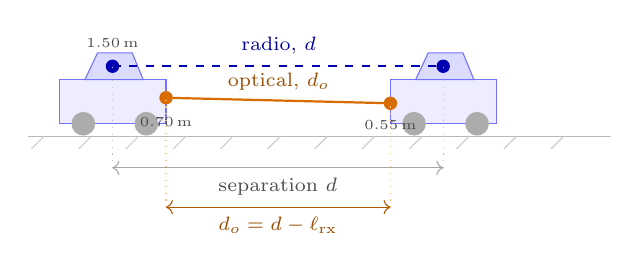
\begin{tikzpicture}[font=\scriptsize, x=1mm, y=1mm]
  % --- side elevation -------------------------------------------------------
  \draw[gray!55] (0,0) -- (74,0);
  \foreach \x in {2,8,...,72} \draw[gray!40] (\x,0) -- (\x-1.6,-1.6);

  % follower
  \draw[fill=blue!7, draw=blue!55] (4,1.6) rectangle (17.5,7.2);
  \draw[fill=blue!14, draw=blue!55] (7.2,7.2) -- (14.6,7.2) -- (13.2,10.6) -- (8.8,10.6) -- cycle;
  \fill[gray!65] (7.0,1.6) circle (1.5); \fill[gray!65] (15.0,1.6) circle (1.5);
  % leader
  \draw[fill=blue!7, draw=blue!55] (46,1.6) rectangle (59.5,7.2);
  \draw[fill=blue!14, draw=blue!55] (49.2,7.2) -- (56.6,7.2) -- (55.2,10.6) -- (50.8,10.6) -- cycle;
  \fill[gray!65] (49.0,1.6) circle (1.5); \fill[gray!65] (57.0,1.6) circle (1.5);

  % endpoints
  \fill[orange!85!black] (17.5,4.9) circle (0.85);
  \fill[orange!85!black] (46,4.2) circle (0.85);
  \fill[blue!70!black]  (10.7,8.9) circle (0.85);
  \fill[blue!70!black]  (52.7,8.9) circle (0.85);

  % links
  \draw[orange!85!black, thick] (17.5,4.9) -- (46,4.2);
  \draw[blue!70!black, thick, dashed] (10.7,8.9) -- (52.7,8.9);

  \node[orange!60!black, anchor=south] at (31.8,4.6) {optical, $d_o$};
  \node[blue!60!black, anchor=south] at (31.8,9.2) {radio, $d$};
  \node[anchor=north, gray!60!black] at (17.5,3.6) {\tiny 0.70\,m};
  \node[anchor=north, gray!60!black] at (46,3.2) {\tiny 0.55\,m};
  \node[anchor=south, gray!60!black] at (10.7,10.0) {\tiny 1.50\,m};

  % the distance that is not the separation
  \draw[<->, gray!70] (10.7,-4) -- (52.7,-4);
  \node[anchor=north, gray!60!black] at (31.7,-4) {separation $d$};
  \draw[<->, orange!70!black] (17.5,-9) -- (46,-9);
  \node[anchor=north, orange!60!black] at (31.7,-9) {$d_o = d - \ell_{\mathrm{rx}}$};
  \draw[gray!50, dotted] (10.7,-4) -- (10.7,8.9);
  \draw[gray!50, dotted] (52.7,-4) -- (52.7,8.9);
  \draw[orange!50, dotted] (17.5,-9) -- (17.5,4.9);
  \draw[orange!50, dotted] (46,-9) -- (46,4.2);
\end{tikzpicture}
\caption{Link geometry for one tagged pair, to scale vertically. The radio runs
centre to centre at \SI{1.5}{\meter}; the optical link runs from the follower's
headlamp at \SI{0.7}{\meter} to the leader's rear-mounted photodiode at
\SI{0.55}{\meter}, and is therefore shorter than the separation by one receiver
length. Because the two paths sit at different heights and different endpoints
they are obstructed by different vehicles, which is what makes their failures
independent. The \SI{0.15}{\meter} drop also sets the vertical emission angle,
$-\arctan(\Delta h/d_o)$, and hence which row of the beam a pair reads.}
\label{fig:geometry}
\end{figure}


The geometry engine computes hidden ground truth. It is used to generate
outcomes and to answer oracle questions; it is never visible to a policy
(Sec.~\ref{sec:arch}).

\subsection{Link endpoints}

Three antenna-like reference points are defined per vehicle: the RF antenna at
the body centre at \SI{1.5}{\meter}, the headlamp at the front face at
\SI{0.7}{\meter}, and the photodiode at the rear face at \SI{0.55}{\meter}.
The optical link path therefore runs headlamp-to-photodiode and is shorter
than the separation by one receiver length, while the radio path runs
centre-to-centre.

\subsection{Pair geometry}

For a transmitter--receiver pair, the engine computes separation $d$, optical
path length $d_o$, world-frame bearing, \emph{signed} relative bearing,
relative heading, headlamp emission angle and photodiode incidence angle
$\psi$. Acceptance at the receiver is the cone test $\psi \le \psi_c$ with
$\psi_c=\SI{60}{\degree}$.

The signed relative bearing is used rather than an absolute emission angle. An
automotive low beam is deliberately asymmetric about its optical axis; feeding
an absolute angle to such a pattern folds its left half onto its right and
silently symmetrises exactly the feature that distinguishes a measured beam
from a cosine lobe.

\subsection{Occlusion and propagation class}

Vehicles are modelled as oriented rectangles. Candidate blockers are retrieved
from a uniform-grid spatial index whose cell size is at least the largest
vehicle diagonal, then tested by segment--rectangle intersection. The radio
path is classified as
\begin{itemize}
\item \textbf{NLOS} if any building rectangle intersects it;
\item \textbf{NLOSv} otherwise, if any vehicle intersects it;
\item \textbf{LOS} otherwise.
\end{itemize}
The optical path is a binary obstructed/clear test. Blocker identities are
returned so that NLOSv blockage depth can be computed from the height of the
\emph{actual} tallest blocker rather than a nominal value.

\section{Sidelink Channel Model}
\label{sec:rf}

The radio operates at \SI{5.9}{\giga\hertz} over \SI{10}{\mega\hertz}, with
\num{24} resource blocks at \SI{30}{\kilo\hertz} subcarrier spacing,
\SI{23}{\dBm} transmit power, 16-QAM, and a \SI{0.5}{\milli\second} slot. The
service profile grants three frequency-hopped attempts per packet.

\subsection{Large-scale path loss}

Path loss follows the TR 37.885 urban family \cite{tr37885}:
\begin{align}
L_{\mathrm{LOS}} &= 38.77 + 16.7\log_{10}d + 18.2\log_{10}f_c,\\
L_{\mathrm{NLOS}} &= 36.85 + 30.0\log_{10}d + 18.9\log_{10}f_c,
\end{align}
with $d$ in metres and $f_c$ in \si{\giga\hertz}. NLOSv adds a blockage term
whose mean depends on blocker height relative to the endpoint antennas and
whose spread is $\sigma=\SI{4.5}{\decibel}$ for tall blockers and
\SI{4.0}{\decibel} for mixed.

\subsection{Spatially correlated shadowing}

Shadowing is correlated in travelled distance following Gudmundson
\cite{gudmundson1991}. With autocorrelation $\rho(\Delta d)=
\exp(-\Delta d/d_{\mathrm{corr}})$, the per-link state evolves as a
first-order autoregression
\begin{equation}
s_{k} = \rho\,s_{k-1} + \sqrt{1-\rho^{2}}\;\mathcal{N}(0,1),
\end{equation}
with $d_{\mathrm{corr}}=\SI{10}{\meter}$ for LOS and NLOSv and
\SI{13}{\meter} for NLOS.

The state is stored at unit variance and scaled by the class-dependent
$\sigma$ only when read. This is deliberate: a link crossing from LOS into
NLOSv has not moved to a different neighbourhood, it has had a vehicle pull in
front of it. Storing $\sigma$-scaled state would make every class transition a
discontinuity in the shadowing itself and would inject an artificial
correlation between the propagation-class sequence and the shadowing
sequence---precisely the correlation the framework exists to measure rather
than manufacture.

\subsection{Small-scale fading}

Fading is correlated in both time and frequency with a separable kernel
$R(\Delta t,\Delta f)=R_t(\Delta t)\,R_f(\Delta f)$. The temporal factor is
Clarke's isotropic-scattering autocorrelation \cite{clarke1968},
\begin{equation}
R_t(\Delta t) = J_0(2\pi f_d \Delta t),
\end{equation}
where the Doppler spread $f_d$ is formed from the \emph{sum} of the two
terminal speeds, both being mobile. The frequency factor follows from an
exponential power--delay profile with RMS delay spread
$\tau_{\mathrm{rms}}=\SI{200}{\nano\second}$, giving the Lorentzian
\begin{equation}
R_f(\Delta f) = \frac{1}{\sqrt{1+(2\pi\,\Delta f\,\tau_{\mathrm{rms}})^{2}}}.
\end{equation}
A Rician specular component with $K=\SI{9}{\decibel}$ is added at read time
for LOS. The three granted attempts are placed at hop offsets spread evenly
across the configured bandwidth; with $\tau_{\mathrm{rms}}=\SI{200}{\nano
\second}$ the subchannels decorrelate to $0.5$ within about
\SI{1.4}{\mega\hertz}, so a \SI{10}{\mega\hertz} band yields three
near-independent hops.

Separability is an approximation and is stated as one: a jointly correlated
scattering model would not factor exactly, but the factored form reproduces
both marginals, which is what the retransmission model reads.

\subsection{Contention}

Resource contention is modelled analytically. Given $N$ contenders within a
\SI{200}{\meter} radius and a resource pool of size $M$, the collision
probability follows a birthday-collision form, augmented with a hidden-terminal
term and a half-duplex term. The model is named in the implementation as an
\emph{analytical collision model with sensitivity bands} and explicitly
\emph{not} as an NR Mode~2 sensing simulation, since no sensing, reservation
or re-selection procedure is simulated. Three parameter bands---optimistic,
nominal and pessimistic---are declared so that conclusions can be reported as
robust or not.

\subsection{Finite-blocklength decoding}

At \SI{300}{\byte} and \SI{3}{\milli\second}, asymptotic capacity flatters the
radio. Block error probability uses the normal approximation of Polyanskiy,
Poor and Verd\'u \cite{ppv2010}: for blocklength $n$, SNR $\gamma$ and error
$\epsilon$, the maximal rate satisfies
\begin{equation}
k \approx nC(\gamma) - \sqrt{nV(\gamma)}\,Q^{-1}(\epsilon)
+ \tfrac{1}{2}\log_2 n,
\end{equation}
with $C=\log_2(1+\gamma)$ and dispersion
$V=\frac{\gamma(\gamma+2)}{(\gamma+1)^{2}}(\log_2 e)^{2}$. Under the headline
profile $n=\num{2419}$ channel uses and $k=\num{2784}$ information bits,
derived from the resource grid and modulation order rather than assumed.

\subsection{Composition}

The RF fa\c{c}ade exposes two operations: evaluate one attempt against a
supplied random tape, and report its failure probability \emph{without}
consuming the tape. The latter is what allows an oracle to price an action it
did not take. An attempt draws three uniforms---collision, decoding and
half-duplex.

\section{V-VLC Channel Model}
\label{sec:vlc}

The optical link uses intensity modulation with direct detection (IM/DD) and
on--off keying at \SI{4.5}{\mega\bit\per\second} gross rate, \SI{2.4}{\milli
\second} airtime, and a single attempt per packet.

\subsection{Headlamp radiant intensity}

The transmitter is characterised by a tabulated radiant-intensity pattern
$I(\theta_h,\theta_v)$ rather than a Lambertian lobe. UN Regulation No.~112 is
a \emph{compliance envelope}, not a beam: it states nine point limits, four
zone limits and eight grouped-point minima, all confined to 9L--9R
horizontally and 4U--4D vertically. Building a pattern directly on those
coordinates yields a sparse scatter of spikes separated by whatever the author
places between them, and interpolating across it produces a shape belonging to
the sampling grid rather than to any lamp.

The artifact is therefore a smooth two-lobe distribution with an asymmetric
cut-off, fitted so that every R112 Class~B limit holds by construction and
verified numerically before the artifact is written; the generator refuses to
emit a non-compliant pattern. Figure~\ref{fig:beam} shows the result against
the limits that constrain it. It is a plausible compliant design and not a
measured lamp, and where measured patterns are available
\cite{alsalami2021,memedi2018} they should replace it.

Beyond 9L/9R the regulation imposes no minimum, so emission there is a design
choice. Two variants ship---one continuing the model's own falloff, one
applying a steeper decay past the last regulated angle---and every result that
depends on the unregulated region is reported as a band across them.

Two further properties are enforced. The pattern refuses extrapolation beyond
its own grid: a direction outside it raises rather than returning an edge
value, and callers must query coverage explicitly. And a Lambertian pattern
exists in the codebase as a named comparison model only, never constructed as
a fallback---a cosine lobe substituted for a real beam would look identical to
a genuine result in every log.


\begin{figure*}[!t]
\centering
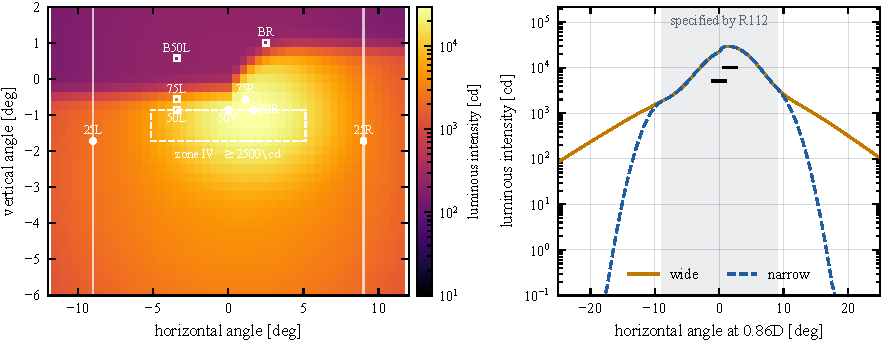
\includegraphics[width=\textwidth]{fig_headlamp_pattern.pdf}
\caption{The modelled beam against the regulation that constrains it.
Left: the pattern with every ECE~R112 Class~B passing-beam test point and the
zone~IV box drawn on it; filled markers carry minima, open markers maxima. The
cut-off and its asymmetric shoulder are the features that distinguish a real
low beam from a cosine lobe. Right: a horizontal cut at 0.86D. The regulation
specifies nothing beyond 9L/9R, so the two shipped variants diverge there by
construction and every result depending on that region is reported as a band
across them.}
\label{fig:beam}
\end{figure*}

\subsection{Optical gain}

Received optical power for an unobstructed, aligned pair is
\begin{equation}
P_r = \frac{I(\theta_h,\theta_v)\;A_{\mathrm{eff}}(\psi)}{d_o^{2}},
\label{eq:optical}
\end{equation}
with effective receiver area
\begin{equation}
A_{\mathrm{eff}}(\psi) = A\,T_s\,g(\psi)\cos\psi,\qquad
g(\psi)=\frac{n^{2}}{\sin^{2}\psi_c},
\end{equation}
for $\psi\le\psi_c$ and zero otherwise \cite{kahn1997}. The implementation
uses $A=\SI{7.5}{\milli\meter\squared}$, responsivity
\SI{0.4}{\ampere\per\watt}, optical filter transmission $T_s=0.9$ and
concentrator index $n=1.5$, with the \emph{same} $\psi_c$ in the gain as in
the acceptance test---a wide cone for availability combined with narrow-cone
gain would count the same physics twice.

The vertical emission angle is $-\arctan(\Delta h/d_o)$ with
$\Delta h=\SI{0.3}{\meter}$, which is \SI{-1.7}{\degree} at a
\SI{10}{\meter} path and steepens rapidly as the pair closes. Below roughly
\SI{0.8}{\meter} it exceeds the pattern envelope. Below the far-field validity
distance of \SI{1}{\meter}, the geometry adapter holds $d_o$ at that floor:
conservative, since $1/d_o^{2}$ then awards less power than the pair has, into
a margin of order \SI{40}{\decibel}.

\subsection{Noise and detection}

Electrical SNR is formed against shot and thermal noise,
\begin{equation}
\gamma = \frac{(R P_r)^{2}}{\sigma^{2}_{\mathrm{shot}}
+ \sigma^{2}_{\mathrm{thermal}}},
\qquad
\sigma^{2}_{\mathrm{shot}} = 2qI_{\mathrm{bg}}B,
\end{equation}
with $I_{\mathrm{bg}}$ the ambient photocurrent. Two named conditions are
defined: clear night at \SI{100}{\nano\ampere} (declared) and clear day at
\SI{3}{\milli\ampere} (derived from \SI{1}{\kilo\watt\per\meter\squared} on
the stated detector). The derived daylight value matters because shot noise
only overtakes thermal at \SI{308}{\micro\ampere}; a smaller assumed figure
never changes the noise regime and would misrepresent the sensitivity.

For OOK against average optical power, $\mathrm{BER}=Q(\sqrt{\gamma})$, and
the coded packet error follows from the block length and code rate with a
correctable-fraction model.

\subsection{Failure taxonomy}

The optical result distinguishes three failure causes, and the distinction is
structural rather than cosmetic:
\begin{itemize}
\item \textbf{Occlusion} --- the path is severed; no power fixes it.
\item \textbf{Alignment} --- either the incidence angle exceeds $\psi_c$
(receiver side) or the emission direction lies outside the beam envelope
(transmitter side).
\item \textbf{Channel} --- the path was clear and aligned but the coded block
did not decode.
\end{itemize}
The first two are \emph{geometric}: immune to any transmit- or receive-power
improvement, and together they define the outage floor $P_{\mathrm{out}}$ that
caps what the optical leg can contribute. Notably, the optical result carries
\emph{no} contention field, and this absence is asserted by test: a
directional point-to-point link has no equivalent of collision, which is the
asymmetry the hybrid case rests upon.

\section{Packet Lifecycle and CMDP Formulation}
\label{sec:cmdp}

\subsection{Actions and cost}

At each packet the system selects one action from
$\mathcal{A}=\{\textsc{rf},\textsc{vlc},\textsc{dup}\}$ with activation costs
$g(\textsc{rf})=g(\textsc{vlc})=1$ and $g(\textsc{dup})=2$. Both legs of a
duplicated packet always pay, even when the radio arrives first and the
optical copy is discarded. This is what makes duplication genuinely expensive
and gives the constraint something to trade against.

\subsection{Deadline arithmetic}

With deadline $D=\SI{3}{\milli\second}$ and a pre-decision lead of
\SI{0.1}{\milli\second}, the available window is \SI{2.9}{\milli\second}. The
two media occupy different physical channels and run concurrently, so the
binding quantity is the longer leg, not the sum:
\begin{equation}
\max\!\left(N_{\mathrm{rf}}\,t_{\mathrm{rf}},\; t_{\mathrm{vlc}}\right)
= \max(3\times 0.5,\;2.4) = \SI{2.4}{\milli\second} \le \SI{2.9}{\milli\second}.
\end{equation}
A profile violating this is refused at construction, so that misses are never
attributable to arithmetic while looking identical to physics in the logs.

\subsection{Matched random tapes}

One random tape is drawn per packet and every action reads from it, so
\textsc{rf}, \textsc{vlc} and \textsc{dup} are evaluated against the same
realised channel. Without this, the difference between two actions on one
packet carries a sampling artefact that no amount of averaging separates from
a real effect at a $10^{-4}$ budget.

The tape is seeded from packet \emph{identity}---the tuple (trace, pair,
packet index)---rather than from a running stream. Consequently, evaluating
one extra action, or visiting pairs in a different order, does not perturb any
other packet's channel realisation.

\subsection{Constrained formulation}

Let $\pi$ be a policy mapping observations to actions, $g$ the activation
cost, and $c_k$ the miss indicator for density group $k$. The problem is
\begin{equation}
\min_{\pi}\;\mathbb{E}_{\pi}\!\left[g\right]
\quad\text{s.t.}\quad
J_{c,k}(\pi) = \mathbb{E}_{\pi}\!\left[c_k\right] \le \delta,\;
\forall k,
\label{eq:cmdp}
\end{equation}
with $\delta=10^{-4}$. This is a constrained MDP \cite{altman1999}, addressed
by primal--dual optimisation: the Lagrangian
$\mathcal{L}(\pi,\lambda)=\mathbb{E}_\pi[g]+\sum_k\lambda_k
(J_{c,k}(\pi)-\delta)$ is minimised over $\pi$ by PPO \cite{schulman2017}
while each $\lambda_k\ge 0$ ascends on constraint violation.

Two design choices are worth stating. The constraint is enforced \emph{per
density group}, so a policy cannot satisfy an average by failing the dense
case and over-delivering in the sparse one. And the cost signal is the
per-packet conditional miss \emph{probability} rather than the realised miss
indicator---at $10^{-4}$ the indicator is almost always zero and carries
almost no gradient.

\section{Software Architecture}
\label{sec:arch}

\begin{figure*}[!t]
\centering
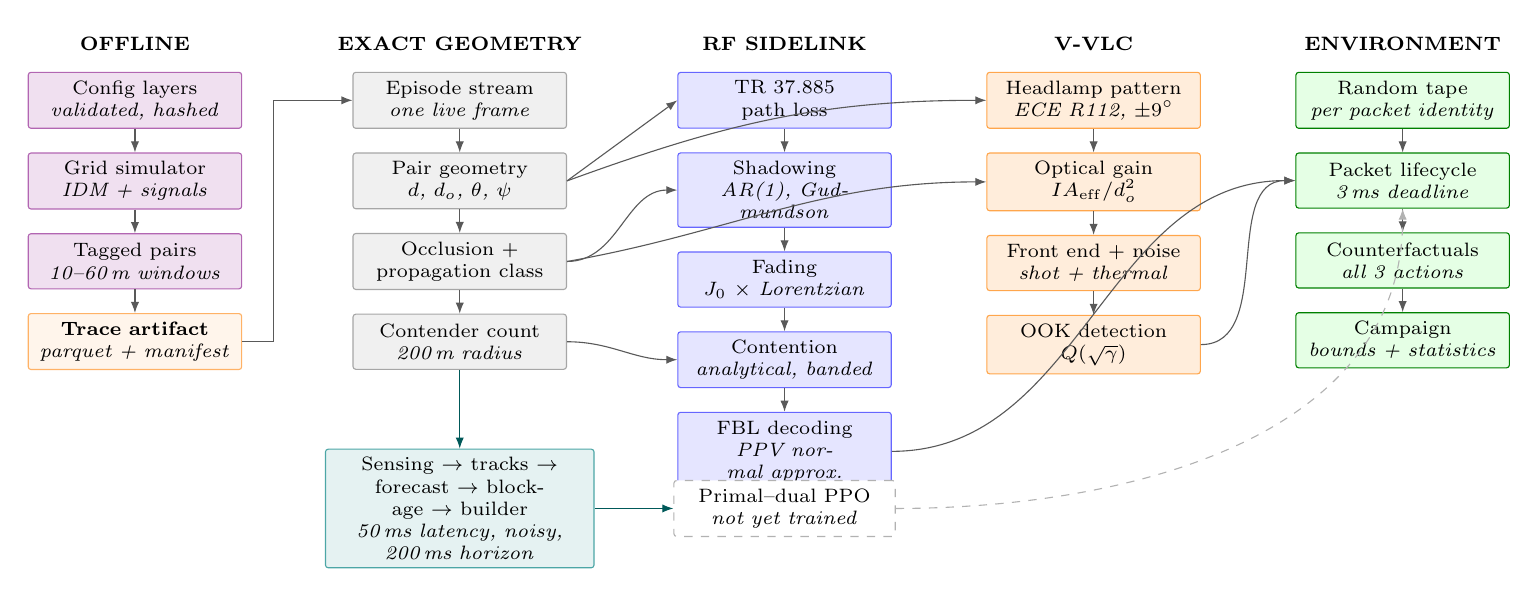
\begin{tikzpicture}[
  font=\scriptsize,
  node distance=3mm,
  box/.style={draw, rounded corners=1pt, align=center, minimum height=7mm,
              inner xsep=3pt, inner ysep=3pt, text width=25mm},
  mob/.style={box, fill=violet!12, draw=violet!60},
  geo/.style={box, fill=gray!12, draw=gray!70},
  rf/.style={box, fill=blue!10, draw=blue!60},
  vlc/.style={box, fill=orange!14, draw=orange!70},
  env/.style={box, fill=green!10, draw=green!50!black},
  obs/.style={box, fill=teal!10, draw=teal!70},
  todo/.style={box, fill=white, draw=gray!60, dashed},
  ar/.style={-{Latex[length=1.4mm]}, gray!70!black},
  lbl/.style={font=\scriptsize\bfseries}
]

% --- offline column
\node[mob] (cfg)  {Config layers\\\textit{validated, hashed}};
\node[mob, below=of cfg] (sim) {Grid simulator\\\textit{IDM + signals}};
\node[mob, below=of sim] (pair) {Tagged pairs\\\textit{10--60\,m windows}};
\node[geo, below=of pair, fill=orange!8, draw=orange!60] (trace)
  {\textbf{Trace artifact}\\\textit{parquet + manifest}};

\node[lbl, above=1.5mm of cfg] {OFFLINE};

% --- geometry column
\node[geo, right=14mm of cfg] (epi) {Episode stream\\\textit{one live frame}};
\node[geo, below=of epi] (pg) {Pair geometry\\\textit{$d$, $d_o$, $\theta$, $\psi$}};
\node[geo, below=of pg] (occ) {Occlusion +\\propagation class};
\node[geo, below=of occ] (cont) {Contender count\\\textit{200\,m radius}};

\node[lbl, above=1.5mm of epi] {EXACT GEOMETRY};

% --- RF column
\node[rf, right=14mm of epi] (pl) {TR 37.885\\path loss};
\node[rf, below=of pl] (sh) {Shadowing\\\textit{AR(1), Gudmundson}};
\node[rf, below=of sh] (fd) {Fading\\\textit{$J_0$ $\times$ Lorentzian}};
\node[rf, below=of fd] (col) {Contention\\\textit{analytical, banded}};
\node[rf, below=of col] (bl) {FBL decoding\\\textit{PPV normal approx.}};

\node[lbl, above=1.5mm of pl] {RF SIDELINK};

% --- VLC column
\node[vlc, right=12mm of pl] (pat) {Headlamp pattern\\\textit{ECE R112, $\pm9^\circ$}};
\node[vlc, below=of pat] (gain) {Optical gain\\\textit{$I A_{\mathrm{eff}}/d_o^2$}};
\node[vlc, below=of gain] (nz) {Front end + noise\\\textit{shot + thermal}};
\node[vlc, below=of nz] (ook) {OOK detection\\\textit{$Q(\sqrt{\gamma})$}};

\node[lbl, above=1.5mm of pat] {V-VLC};

% --- env column
\node[env, right=12mm of pat] (tape) {Random tape\\\textit{per packet identity}};
\node[env, below=of tape] (life) {Packet lifecycle\\\textit{3\,ms deadline}};
\node[env, below=of life] (cf) {Counterfactuals\\\textit{all 3 actions}};
\node[env, below=of cf] (camp) {Campaign\\\textit{bounds + statistics}};

\node[lbl, above=1.5mm of tape] {ENVIRONMENT};

% --- observation / policy
\node[obs, below=10mm of cont, text width=32mm] (obsb)
  {Sensing $\to$ tracks $\to$ forecast $\to$ blockage $\to$ builder\\
   \textit{50\,ms latency, noisy, 200\,ms horizon}};
\node[todo, right=10mm of obsb, text width=26mm] (pol)
  {Primal--dual PPO\\\textit{not yet trained}};

% --- edges
\draw[ar] (cfg) -- (sim);
\draw[ar] (sim) -- (pair);
\draw[ar] (pair) -- (trace);
\draw[ar] (trace.east) -- ++(4mm,0) |- (epi.west);
\draw[ar] (epi) -- (pg);
\draw[ar] (pg) -- (occ);
\draw[ar] (occ) -- (cont);

\draw[ar] (pg.east) -- (pl.west);
\draw[ar] (occ.east) to[out=0,in=180] (sh.west);
\draw[ar] (cont.east) to[out=0,in=180] (col.west);

\draw[ar] (pl) -- (sh);
\draw[ar] (sh) -- (fd);
\draw[ar] (fd) -- (col);
\draw[ar] (col) -- (bl);

\draw[ar] (pg.east) to[out=20,in=180] (pat.west);
\draw[ar] (occ.east) to[out=10,in=180] (gain.west);
\draw[ar] (pat) -- (gain);
\draw[ar] (gain) -- (nz);
\draw[ar] (nz) -- (ook);

\draw[ar] (bl.east) to[out=0,in=180] (life.west);
\draw[ar] (ook.east) to[out=0,in=180] (life.west);
\draw[ar] (tape) -- (life);
\draw[ar] (life) -- (cf);
\draw[ar] (cf) -- (camp);

\draw[ar, teal!70!black] (cont.south) -- (obsb.north);
\draw[ar, teal!70!black] (obsb) -- (pol);
\draw[ar, gray!60, dashed] (pol.east) to[out=0,in=270] (life.south);

\end{tikzpicture}
\caption{GRAIL-V block architecture. The offline pipeline (left) produces a
mobility trace on disk; the online pipeline replays it, rebuilding exact
geometry per packet and driving both channel models from the same pair pose.
The two channels are composed by the packet lifecycle under a
\SI{3}{\milli\second} deadline against one shared random tape, so that all
three actions are evaluated on the same realised channel. The observation
chain (bottom) is the only path a deployable policy may read: exact geometry
reaches the channels but never the policy.}
\label{fig:arch}
\end{figure*}

Fig.~\ref{fig:arch} shows the composition. The implementation comprises 71
modules and approximately \num{15500} lines with \num{725} unit tests. It is
organised in layers with a strict dependency direction: foundations
(determinism, configuration, artifact provenance), mobility, geometry, the two
channel models, and the environment. The packet lifecycle deliberately
contains \emph{no channel equations}; both fa\c{c}ades answer the same two
questions, so the lifecycle only sequences them and applies the deadline.

\subsection{The information barrier}

The single most load-bearing structural property is that exact geometry must
not reach a deployable policy. Vehicle state forks into two paths:

\begin{itemize}
\item \textbf{Exact path.} Geometry $\rightarrow$ channels $\rightarrow$
outcome generation and oracle queries.
\item \textbf{Causal path.} Sensing (\SI{50}{\milli\second} update and
latency; $\sigma=\SI{0.5}{\meter}$, \SI{0.2}{\meter\per\second},
\SI{2}{\degree}) $\rightarrow$ track store (\SI{1}{\second} lifetime)
$\rightarrow$ \SI{200}{\milli\second} constant-velocity forecast $\rightarrow$
blockage probability with confidence $\rightarrow$ a 21-feature observation
vector with 8-packet history.
\end{itemize}

The barrier is enforced three ways, because it can fail three ways: the
configuration cannot \emph{name} a forbidden observation field; an
abstract-syntax-tree import guard prevents the observation layer from reaching
the geometry layer; and the forbidden quantities are enumerated by name so
that a future field smuggling one in under an alias is caught by review.

\subsection{Reproducibility}

Every artifact carries a manifest with a SHA-256 digest per file, the
configuration hash, the code commit and the random seeds, and is re-verified
on read. Configuration hashing is \emph{scoped}: a change to a channel
parameter does not invalidate mobility traces, which is what makes an
iterative channel study affordable against a 21-trace campaign. Randomness is
drawn from named independent streams so that adding a channel draw cannot
shift the mobility sequence.

\section{Evaluation Methodology}
\label{sec:method}

A $10^{-4}$ target changes what counts as evidence, and three methodological
choices follow from it.

\subsection{The constraint is an expectation, so it is estimated as one}

Verifying $10^{-4}$ by counting realised misses requires on the order of
$10^{6}$ packets per density before the count is even stable. The per-packet
failure probability is available exactly from both fa\c{c}ades, and its sample
mean estimates the same quantity with far smaller variance. Both are reported:
the expectation is the estimate, and the realised count is the check that the
expectation is not lying.

The realised-rate resampling bound has a hard limitation at this budget. With
zero observed misses it returns zero, because resampling clusters that all
contain no miss can only produce no miss; rendered as a 95\,\% bound, that
reads as certainty. The expectation has no such failure mode, since every
packet carries a probability whether or not it failed.

\subsection{Packets are not independent samples}

Every packet within one tagged-pair episode shares that pair's shadowing
state, fading trajectory, geometry and very nearly its contention. The
effective sample size is therefore the number of episodes. Confidence bounds
resample whole episode \emph{clusters} with replacement and recompute the rate
as a ratio of sums---not a mean of per-cluster rates, since episodes differ in
length by an order of magnitude \cite{cameron2015}.

All bounds are \textbf{one-sided upper at 95\,\%}, i.e. $z=1.6449$. This is
stated explicitly because it is decision-relevant: at the highest density the
realised duplication rate bounds to $9.70\times10^{-5}$ at $z=1.6449$ and
$1.005\times10^{-4}$ at $z=1.96$, so the same data passes or fails the budget
depending on which convention is meant. The Wilson score interval
\cite{wilson1927} is retained alongside the resampled bound for comparison;
Poisson counts use the Garwood exact interval \cite{garwood1936}.

\subsection{Two bounds, answering different questions}

\paragraph{Realisation oracle} chooses the cheapest action that delivers on
each realised packet. It misses only when \emph{no} action would have
delivered---exactly duplication's failure event---so its reliability equals
duplication's while its cost approaches unity. It is an upper bound on
achievable performance that no causal policy can approach, since it conditions
on the outcome.

\paragraph{Targeting bound} answers the question a learner can actually
address: what if a policy knew each packet's failure \emph{probability} but
still had to choose before the draw? Duplicating packet $i$ costs one extra
unit and reduces expected miss by $p_{\mathrm{rf},i}-p_{\mathrm{joint},i}$.
Since every packet costs the same, the greedy solution is exact---sort by
reduction and duplicate from the top until the mean expected miss falls under
$\delta$. Sweeping $\delta$ traces a reliability--cost frontier.

This bound is the meaningful target for the policy-optimisation stage. If it
sat near $2.0$, per-packet risk would be too flat to target and no policy
could beat blind duplication; if near $1.0$, risk is concentrated and there is
real headroom.

\section{Measured Results}
\label{sec:results}

Results below are from the held-out test split, pooled across three replicate
traces with a \SI{400}{\second} warm-up discarded. The warm-up is necessary
because a trace opens in its seeded formation---evenly spaced and
aligned---and is unrepresentative until the traffic disperses.

Densities 10 and 20 use \num{1000000} packets per density; density 30 uses
\num{3000000}, and the difference is a finding rather than a convenience. At
\num{1000000} packets the density-30 result twice fell on the wrong side of
the constraint and twice reversed at \num{3000000}. The mechanism is that a
denser frame yields more pairs, so a packet budget is exhausted after far less
simulated time: \num{1000000} packets bought \num{6484} pair episodes at
density 30, while \num{3000000} bought \num{12899}. The sample was not merely
smaller, it was less mixed. \textbf{The sufficiency criterion should therefore
be independent episodes, not packets}---a study reproducing this at a
\num{1000000}-packet floor would draw the opposite conclusion at the density
that matters most.

\begin{table}[!t]
\caption{Expected miss rate by density and headlamp variant (test split).
Bounds are one-sided upper at 95\,\%; the constraint is judged against the
bound, not the point estimate.}
\label{tab:reliability}
\centering
\begin{tabular}{@{}llS[table-format=1.3e1]S[table-format=1.3e1]c@{}}
\toprule
$\rho$ & policy & {$\mathbb{E}[\text{miss}]$} & {95\,\% upper} & {holds} \\
\midrule
\multirow{3}{*}{10} & RF only & 3.648e-5 & 3.679e-5 & yes \\
 & VLC only & 5.423e-1 & 5.504e-1 & no \\
 & DUP & 2.046e-5 & 2.083e-5 & yes \\
\midrule
\multirow{3}{*}{20} & RF only & 1.803e-4 & 1.831e-4 & no \\
 & VLC only & 3.474e-1 & 3.564e-1 & no \\
 & DUP & 5.913e-5 & 6.115e-5 & yes \\
\midrule
\multirow{3}{*}{30} & RF only & 4.347e-4 & 4.389e-4 & no \\
 & VLC only & 2.301e-1 & 2.354e-1 & no \\
 & DUP (wide) & 9.076e-5 & 9.330e-5 & yes \\
 & DUP (narrow) & 9.675e-5 & 9.943e-5 & yes \\
\bottomrule
\end{tabular}
\end{table}


\begin{figure}[!t]
\centering
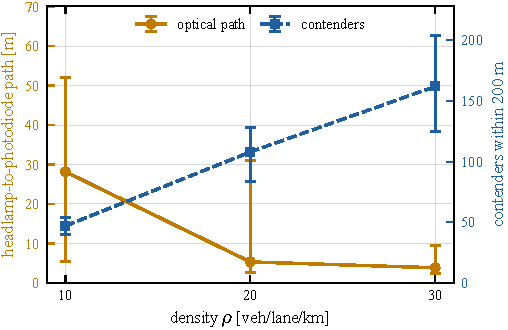
\includegraphics[width=\columnwidth]{fig_coupling.pdf}
\caption{The coupling the contribution rests on. Optical path length and
contender count are measured over the same tagged-pair instants of the same
traces, so their opposition is a property of one traffic state rather than of
two independently parameterised models. Markers are medians, bars the
interquartile range. The curves cross near $\rho=17$: below it the light has
the harder job, above it the radio does.}
\label{fig:coupling}
\end{figure}

\subsection{Neither medium suffices alone}

Table~\ref{tab:reliability} shows the radio meeting the budget only at the
lowest density; at $\rho=20$ and $\rho=30$ its upper bound exceeds $10^{-4}$ by
$1.8\times$ and $4.4\times$. The optical link alone fails everywhere by three
orders of magnitude, dominated not by decoding but by range and geometry.

Duplication meets the budget at every density on the bound, and---the point of
carrying two variants---it does so under both headlamp assumptions. The margin
is thin where it matters: at $\rho=30$ the bound clears by $6.7\%$ under the
wide variant and by $0.57\%$ under the narrow one. The reliability of a
headlamp-based optical link at high density therefore rests on emission the
regulation does not require, and the honest statement is that the constraint is
met across the range of compliant designs rather than met with margin.


\begin{figure}[!t]
\centering
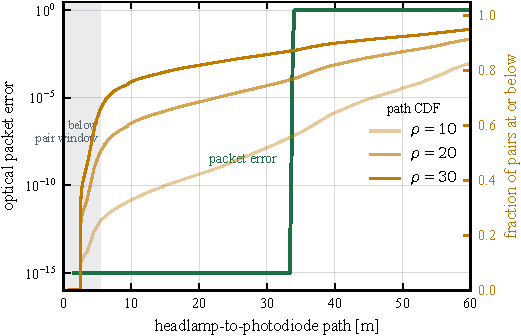
\includegraphics[width=\columnwidth]{fig_optical_cliff.pdf}
\caption{The optical link is decided by range, and density decides the
range. An inverse-square budget against a steep coded threshold puts the whole
transition within a few metres of \SI{34}{\meter}, so the packet-error curve is
nearly binary. Overlaid with the measured distribution of optical path at each
density it explains the optical column of Table~\ref{tab:reliability}: at
$\rho=10$ the median pair sits at \SI{28.2}{\meter} and most of the
distribution is past the cliff, while at $\rho=30$ the median is
\SI{3.8}{\meter} and nearly all of it is inside. Shading marks paths shorter
than the tagged-pair admission window admits.}
\label{fig:cliff}
\end{figure}

\subsection{The failures are independent}

The dependence ratio $p_{\mathrm{joint}}/(p_{\mathrm{rf}}\,p_{\mathrm{vlc}})$
equals unity under independence. Pooled over the campaign it is $0.923$ with a
$95\%$ Poisson interval of $[0.826, 1.029]$, from \num{325} realised joint
failures against \num{352} predicted. Per density the values are $0.782$,
$0.929$ and $0.933$, and the narrow variant gives $0.884$, $0.924$ and $0.964$.
The interval brackets unity under either assumption: within the resolution of
several hundred events, the two media fail independently.

This is a measurement of an assumption that comparable studies generally make
silently, and there is a mechanism behind it---radio failure is
collision-dominated, and contention does not care about the geometry that
blocks light.


\begin{figure*}[!t]
\centering
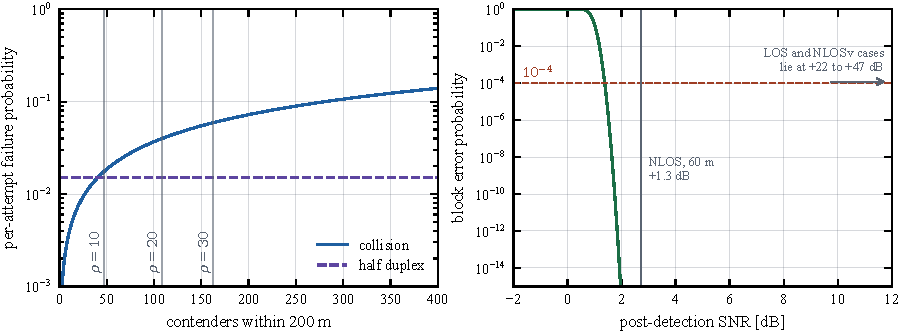
\includegraphics[width=\textwidth]{fig_rf_decomposition.pdf}
\caption{Why the radio's design lever is not its link budget. Left: the
access-layer mechanisms against contention; collision rises with the number of
contenders and half duplex is a flat duty cycle, and neither responds to
transmit power. They cross near \num{45} contenders, which is where $\rho=10$
sits. Right: the finite-blocklength decoding curve. At $n=\num{2419}$ channel
uses it is a cliff about a decibel wide, and the link sits far above it in
every condition except deep NLOS shadowing at the far end of the pair window.
Decoding is negligible because the threshold is sharp and rarely approached,
not because the margin is uniformly large.}
\label{fig:rf}
\end{figure*}

\subsection{The optical leg is range-limited before it is geometry-limited}

\begin{table}[!t]
\caption{Optical outage and complementarity. $P_{\mathrm{out}}$ is identical
across variants---they cover the same directions and differ in how much light
reaches them---so the band appears in the total failure rate, not the floor.}
\label{tab:optical}
\centering
\begin{tabular}{@{}lS[table-format=2.2]S[table-format=2.2]S[table-format=2.2]S[table-format=4.0]@{}}
\toprule
& & \multicolumn{2}{c}{total optical failure [\%]} & \\
\cmidrule(lr){3-4}
$\rho$ & {$P_{\mathrm{out}}$ [\%]} & {wide} & {narrow} & {saved} \\
\midrule
10 & 15.60 & 54.23 & 57.22 & 21 \\
20 & 14.62 & 34.74 & 36.97 & 120 \\
30 & 11.14 & 23.02 & 24.62 & 1049 \\
\bottomrule
\end{tabular}
\end{table}

Table~\ref{tab:optical} separates the geometric floor from total optical
failure. $P_{\mathrm{out}}$ is identical across the two headlamp variants,
which is informative rather than suspicious: both cover the same angular
domain and differ only in how much light reaches its outer part, so the
variant band appears in the link budget and not in the outage floor. The
optical leg is range-limited rather than geometry-limited at low density---at
$\rho=10$ a $15.6\%$ floor sits under a $54\%$ total failure rate---and the two
converge as traffic densifies and pairs close.

The final column gives the complementarity: packets the radio lost and the
light saved, rising from \num{21} to \num{1049} as density increases. This is
the hybrid's reason to exist expressed as a rate, and its growth with density
reflects the structural anti-correlation the framework was built to expose:
the optical path shortens as traffic slows (median \SIrange{26.4}{3.9}{\meter}
from $\rho=10$ to $\rho=30$) exactly as radio contention worsens.


\begin{figure}[!t]
\centering
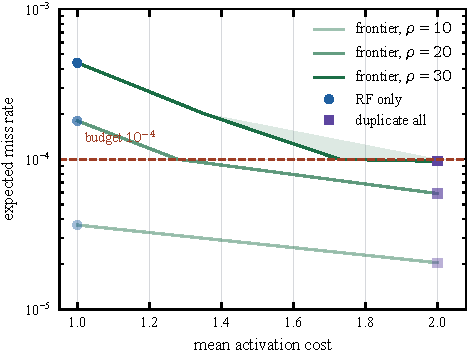
\includegraphics[width=\columnwidth]{fig_frontier.pdf}
\caption{The reliability--cost frontier. Each curve is the cheapest mean
activation cost attaining a given expected miss rate, given perfect knowledge
of per-packet risk but none of outcomes; markers give the two fixed baselines.
The shaded band between headlamp variants is the part of the answer ECE~R112
does not fix. Duplication over-delivers at every density and the frontier
reaches the budget well short of cost~2.}
\label{fig:frontier}
\end{figure}

\subsection{Blind duplication is wasteful}

\begin{table}[!t]
\caption{Targeting bound: mean activation cost at $\delta=10^{-4}$, against
duplication's 2.00}
\label{tab:frontier}
\centering
\begin{tabular}{@{}lS[table-format=1.3]S[table-format=1.3]S[table-format=1.3]@{}}
\toprule
variant & {$\rho=10$} & {$\rho=20$} & {$\rho=30$}\\
\midrule
wide & 1.000 & 1.279 & 1.694\\
narrow & 1.000 & 1.282 & 1.720\\
\bottomrule
\end{tabular}
\end{table}

Table~\ref{tab:frontier} gives the targeting bound at the headline budget:
$1.000$, $1.279$ and $1.694$ against duplication's $2.00$---about a third of
activations recoverable on average, and $15\%$ at the binding density. It is
insensitive to the headlamp variant, moving by at most $0.026$, because it is
driven by the spread of \emph{radio} risk across packets rather than by the
optical budget. The bound is strongly density-dependent, which is the case for
a geometry-aware policy rather than for a fixed strategy.

Two qualifications belong with this number. It assumes perfect knowledge of
per-packet risk, whereas a policy sees a noisy \SI{200}{\milli\second}
forecast; and risk concentration is mild (the riskiest $10\%$ of packets carry
roughly $23\%$ of expected misses), so the headroom is real but not dramatic.

\section{Limitations and Threats to Validity}
\label{sec:limits}

\subsection{Contention is analytical}

No Mode~2 sensing, reservation or re-selection procedure is simulated. The
collision model is analytical with declared sensitivity bands, and it is named
as such throughout the implementation. Cross-validation against a
system-level simulator remains outstanding.

\subsection{Vehicle blockage is weaker than the NLOSv label suggests}

The NLOSv blockage term is decided by comparing the blocker's roof with the two
antennas. With both antennas at \SI{1.5}{\meter} the ``between the antennas''
case cannot fire at all, and the shortest vehicle class is itself
\SI{1.5}{\meter}, so a passenger car---$90\%$ of the fleet---contributes
\emph{zero} additional loss while still being classified NLOSv. A van or truck
contributes a flat \SI{9}{\decibel}: the distance-growth term in the model only
becomes positive beyond \SI{541}{\meter}, far outside the
\SIrange{10}{60}{\meter} tagged-pair window. NLOSv therefore differs from LOS
mainly through the Rician $K$ factor. This is immaterial to the reported
results---radio failure is collision-dominated by two to four orders of
magnitude, so a few decibels either way does not move the miss rate---but the
vehicle-blockage mechanism is weaker in this implementation than the
propagation-class label implies.

\subsection{The optical coding model is conservative by roughly 40\% of range}

The coded packet error assumes bounded-distance decoding correcting $5\%$ of
coded bits at rate $1/4$. The Shannon limit for that rate on a binary symmetric
channel is $21.5\%$, and a capacity-approaching code would extend the optical
range from \SIrange{34}{49}{\meter}. The declared value is therefore at the
pessimistic end of the plausible interval, which is the safe direction for a
claim that the hybrid is necessary, and it is reported as a sensitivity rather
than as a property of any specific code.

\subsection{Sensing coverage is assumed complete}

The collision model separates \emph{where} contenders are from \emph{how well}
sensing works once they are heard. The second is a declared band; the first is
held at unity, meaning every contender within the contention radius is assumed
to have a decodable reservation. A contender behind a building does not, so real
hidden-terminal counts are higher and collisions worse than reported. Deriving
it would require a visibility classification per contender per packet---several
hundred ray casts where the model currently performs two---and it is deferred on
that basis. The pessimistic sensitivity band covers part of the same ground.

\subsection{The headlamp pattern is modelled, not measured}

UN Regulation No.~112 is a compliance envelope, not a beam. It states nine
point limits, four zone limits and eight grouped-point minima, all confined to
9L--9R horizontally and 4U--4D vertically. A pattern built directly on those
points is a sparse scatter of spikes separated by whatever the author places
between them, and interpolating across it yields a beam shape that is an
artefact of the sampling grid. The artifact used here is instead a smooth
two-lobe distribution with an asymmetric cut-off, fitted so that every R112
Class~B limit is satisfied by construction and verified numerically before the
artifact is emitted. It is a plausible compliant design, not a measured lamp,
and where measured patterns are available \cite{alsalami2021,memedi2018} they
should replace it.

Outside 9L--9R the regulation imposes no minimum, so what is emitted there is a
design choice rather than a requirement. Two variants are therefore shipped---
one continuing the model's own falloff, one applying a steeper decay past the
last regulated angle---and results that depend on the unregulated region are
reported as a band across them.

The receiver height interacts with this directly. The vertical emission angle
is $-\arctan(\Delta h/d_o)$, so a large endpoint height difference drives short-
range pairs below 4D, where the regulation says nothing at all---neither floor
nor ceiling. At an earlier \SI{0.40}{\meter} photodiode the drop was
\SI{0.30}{\meter}, 4D was reached at \SI{4.29}{\meter}, and $56\%$ of
density-30 pair-instants sampled directions the regulation does not describe.
The configured \SI{0.55}{\meter} gives a \SI{0.15}{\meter} drop, reaching 4D at
\SI{2.15}{\meter}---below the IDM's minimum gap---so essentially every pair is
sampled inside the regulated domain, and at \SI{10}{\meter} the link reads the
50V/50R hot-spot row.

\subsection{Unsourced parameters}

Eight parameters in the provenance table are recorded as unsourced, including
the shadowing decorrelation distances, the receiver field of view, the
far-field validity distance and the correctable-fraction coding model. Each is
plausible and each is declared.

\subsection{Modelling gaps}

Roads are planar; there is no grade or braking-pitch model, so the vertical
emission angle derives only from the fixed endpoint height difference.
Signal offsets are staggered rather than progressed. Leader vehicle length
varies the optical budget by roughly \SI{4.7}{\decibel} between a car and a
bus, and the observation vector carries no vehicle class, so this variation is
unobservable to a policy.

\subsection{The policy is not trained}

The constrained optimisation stage is fully specified---five seeds,
$10^{7}$ transitions each, per-density multipliers, a curriculum relaxing the
budget from $10^{-2}$ to $10^{-4}$---but not executed. All results in
Sec.~\ref{sec:results} are baselines and bounds. No claim is made here about
what a learned policy achieves.

\section{Conclusion}

GRAIL-V provides an environment in which the RF and V-VLC channels are driven
by one urban traffic state, making their complementarity measurable rather
than assumed. On a held-out test split the measurements are unambiguous: the
sidelink alone misses a $10^{-4}$ budget above the lightest density,
duplication meets it everywhere at twice the activation cost, and the two
media fail approximately independently, with a pooled dependence ratio of
$0.923$ $[0.826,1.029]$.

The framework's more useful output is the targeting bound. It establishes,
without training any policy, that between $31\%$ and $100\%$ of duplication's
excess cost is recoverable by a policy able to predict per-packet risk---and
that the recoverable fraction depends strongly on density, from the whole of it
at $\rho=10$ to roughly a third at $\rho=30$. That is the
quantity against which the constrained policy-optimisation stage should be
judged, and it exists because the environment can evaluate every action on the
same realised packet.

\section*{Acknowledgment}

This report documents an implementation whose parameter provenance is tracked
explicitly; sourced, derived and unsourced values are distinguished in the
project's provenance table and reflected in the limitations above.

\begin{thebibliography}{00}

\bibitem{tr38913} 3GPP, ``Study on scenarios and requirements for next
generation access technologies,'' TR 38.913.

\bibitem{tr37885} 3GPP, ``Study on evaluation methodology of new
Vehicle-to-Everything (V2X) use cases for LTE and NR,'' TR 37.885.

\bibitem{treiber2000} M. Treiber, A. Hennecke, and D. Helbing, ``Congested
traffic states in empirical observations and microscopic simulations,''
\emph{Phys. Rev. E}, vol. 62, no. 2, pp. 1805--1824, 2000.

\bibitem{gudmundson1991} M. Gudmundson, ``Correlation model for shadow fading
in mobile radio systems,'' \emph{Electron. Lett.}, vol. 27, no. 23,
pp. 2145--2146, 1991.

\bibitem{clarke1968} R. H. Clarke, ``A statistical theory of mobile-radio
reception,'' \emph{Bell Syst. Tech. J.}, vol. 47, no. 6, pp. 957--1000, 1968.

\bibitem{ppv2010} Y. Polyanskiy, H. V. Poor, and S. Verd\'u, ``Channel coding
rate in the finite blocklength regime,'' \emph{IEEE Trans. Inf. Theory},
vol. 56, no. 5, pp. 2307--2359, 2010.

\bibitem{kahn1997} J. M. Kahn and J. R. Barry, ``Wireless infrared
communications,'' \emph{Proc. IEEE}, vol. 85, no. 2, pp. 265--298, 1997.

\bibitem{memedi2018} A. Memedi, C. Tebruegge, J. Jahneke, and F. Dressler,
``Impact of vehicle type and headlight characteristics on vehicular VLC
performance,'' in \emph{Proc. 10th IEEE Veh. Netw. Conf. (VNC)}, Taipei,
Taiwan, Dec. 2018.

\bibitem{alsalami2021} F. M. Alsalami \emph{et al.}, ``Impact of vehicle
headlights radiation pattern on dynamic vehicular VLC channel,''
\emph{J. Lightw. Technol.}, vol. 39, no. 10, pp. 3162--3168, 2021.

\bibitem{altman1999} E. Altman, \emph{Constrained Markov Decision Processes}.
Boca Raton, FL: Chapman \& Hall/CRC, 1999.

\bibitem{schulman2017} J. Schulman, F. Wolski, P. Dhariwal, A. Radford, and
O. Klimov, ``Proximal policy optimization algorithms,'' arXiv:1707.06347,
2017.

\bibitem{cameron2015} A. C. Cameron and D. L. Miller, ``A practitioner's guide
to cluster-robust inference,'' \emph{J. Human Resources}, vol. 50, no. 2,
pp. 317--372, 2015.

\bibitem{wilson1927} E. B. Wilson, ``Probable inference, the law of
succession, and statistical inference,'' \emph{J. Amer. Statist. Assoc.},
vol. 22, no. 158, pp. 209--212, 1927.

\bibitem{garwood1936} F. Garwood, ``Fiducial limits for the Poisson
distribution,'' \emph{Biometrika}, vol. 28, no. 3--4, pp. 437--442, 1936.

\end{thebibliography}

\end{document}
